\documentclass[]{article}
\usepackage{lmodern}
\usepackage{amssymb,amsmath}
\usepackage{ifxetex,ifluatex}
\usepackage{fixltx2e} % provides \textsubscript
\ifnum 0\ifxetex 1\fi\ifluatex 1\fi=0 % if pdftex
  \usepackage[T1]{fontenc}
  \usepackage[utf8]{inputenc}
\else % if luatex or xelatex
  \ifxetex
    \usepackage{mathspec}
  \else
    \usepackage{fontspec}
  \fi
  \defaultfontfeatures{Ligatures=TeX,Scale=MatchLowercase}
\fi
% use upquote if available, for straight quotes in verbatim environments
\IfFileExists{upquote.sty}{\usepackage{upquote}}{}
% use microtype if available
\IfFileExists{microtype.sty}{%
\usepackage{microtype}
\UseMicrotypeSet[protrusion]{basicmath} % disable protrusion for tt fonts
}{}
\usepackage{hyperref}
\hypersetup{unicode=true,
            pdfborder={0 0 0},
            breaklinks=true}
\urlstyle{same}  % don't use monospace font for urls
\usepackage{color}
\usepackage{fancyvrb}
\newcommand{\VerbBar}{|}
\newcommand{\VERB}{\Verb[commandchars=\\\{\}]}
\DefineVerbatimEnvironment{Highlighting}{Verbatim}{commandchars=\\\{\}}
% Add ',fontsize=\small' for more characters per line
\newenvironment{Shaded}{}{}
\newcommand{\KeywordTok}[1]{\textcolor[rgb]{0.00,0.44,0.13}{\textbf{{#1}}}}
\newcommand{\DataTypeTok}[1]{\textcolor[rgb]{0.56,0.13,0.00}{{#1}}}
\newcommand{\DecValTok}[1]{\textcolor[rgb]{0.25,0.63,0.44}{{#1}}}
\newcommand{\BaseNTok}[1]{\textcolor[rgb]{0.25,0.63,0.44}{{#1}}}
\newcommand{\FloatTok}[1]{\textcolor[rgb]{0.25,0.63,0.44}{{#1}}}
\newcommand{\ConstantTok}[1]{\textcolor[rgb]{0.53,0.00,0.00}{{#1}}}
\newcommand{\CharTok}[1]{\textcolor[rgb]{0.25,0.44,0.63}{{#1}}}
\newcommand{\SpecialCharTok}[1]{\textcolor[rgb]{0.25,0.44,0.63}{{#1}}}
\newcommand{\StringTok}[1]{\textcolor[rgb]{0.25,0.44,0.63}{{#1}}}
\newcommand{\VerbatimStringTok}[1]{\textcolor[rgb]{0.25,0.44,0.63}{{#1}}}
\newcommand{\SpecialStringTok}[1]{\textcolor[rgb]{0.73,0.40,0.53}{{#1}}}
\newcommand{\ImportTok}[1]{{#1}}
\newcommand{\CommentTok}[1]{\textcolor[rgb]{0.38,0.63,0.69}{\textit{{#1}}}}
\newcommand{\DocumentationTok}[1]{\textcolor[rgb]{0.73,0.13,0.13}{\textit{{#1}}}}
\newcommand{\AnnotationTok}[1]{\textcolor[rgb]{0.38,0.63,0.69}{\textbf{\textit{{#1}}}}}
\newcommand{\CommentVarTok}[1]{\textcolor[rgb]{0.38,0.63,0.69}{\textbf{\textit{{#1}}}}}
\newcommand{\OtherTok}[1]{\textcolor[rgb]{0.00,0.44,0.13}{{#1}}}
\newcommand{\FunctionTok}[1]{\textcolor[rgb]{0.02,0.16,0.49}{{#1}}}
\newcommand{\VariableTok}[1]{\textcolor[rgb]{0.10,0.09,0.49}{{#1}}}
\newcommand{\ControlFlowTok}[1]{\textcolor[rgb]{0.00,0.44,0.13}{\textbf{{#1}}}}
\newcommand{\OperatorTok}[1]{\textcolor[rgb]{0.40,0.40,0.40}{{#1}}}
\newcommand{\BuiltInTok}[1]{{#1}}
\newcommand{\ExtensionTok}[1]{{#1}}
\newcommand{\PreprocessorTok}[1]{\textcolor[rgb]{0.74,0.48,0.00}{{#1}}}
\newcommand{\AttributeTok}[1]{\textcolor[rgb]{0.49,0.56,0.16}{{#1}}}
\newcommand{\RegionMarkerTok}[1]{{#1}}
\newcommand{\InformationTok}[1]{\textcolor[rgb]{0.38,0.63,0.69}{\textbf{\textit{{#1}}}}}
\newcommand{\WarningTok}[1]{\textcolor[rgb]{0.38,0.63,0.69}{\textbf{\textit{{#1}}}}}
\newcommand{\AlertTok}[1]{\textcolor[rgb]{1.00,0.00,0.00}{\textbf{{#1}}}}
\newcommand{\ErrorTok}[1]{\textcolor[rgb]{1.00,0.00,0.00}{\textbf{{#1}}}}
\newcommand{\NormalTok}[1]{{#1}}
\usepackage{longtable,booktabs}
\usepackage{graphicx,grffile}
\makeatletter
\def\maxwidth{\ifdim\Gin@nat@width>\linewidth\linewidth\else\Gin@nat@width\fi}
\def\maxheight{\ifdim\Gin@nat@height>\textheight\textheight\else\Gin@nat@height\fi}
\makeatother
% Scale images if necessary, so that they will not overflow the page
% margins by default, and it is still possible to overwrite the defaults
% using explicit options in \includegraphics[width, height, ...]{}
\setkeys{Gin}{width=\maxwidth,height=\maxheight,keepaspectratio}
\IfFileExists{parskip.sty}{%
\usepackage{parskip}
}{% else
\setlength{\parindent}{0pt}
\setlength{\parskip}{6pt plus 2pt minus 1pt}
}
\setlength{\emergencystretch}{3em}  % prevent overfull lines
\providecommand{\tightlist}{%
  \setlength{\itemsep}{0pt}\setlength{\parskip}{0pt}}
\setcounter{secnumdepth}{0}
% Redefines (sub)paragraphs to behave more like sections
\ifx\paragraph\undefined\else
\let\oldparagraph\paragraph
\renewcommand{\paragraph}[1]{\oldparagraph{#1}\mbox{}}
\fi
\ifx\subparagraph\undefined\else
\let\oldsubparagraph\subparagraph
\renewcommand{\subparagraph}[1]{\oldsubparagraph{#1}\mbox{}}
\fi

\date{}

\begin{document}

\section{Built-In Data Structures}\label{built-in-data-structures}

We have seen Python's simple types: \texttt{int}, \texttt{float},
\texttt{complex}, \texttt{bool}, \texttt{str}, and so on. Python also
has several built-in compound types, which act as containers for other
types. These compound types are:

\begin{longtable}[c]{@{}lll@{}}
\toprule
Type Name & Example & Description\tabularnewline
\midrule
\endhead
\texttt{list} & \texttt{{[}1,\ 2,\ 3{]}} & Ordered
collection\tabularnewline
\texttt{tuple} & \texttt{(1,\ 2,\ 3)} & Immutable ordered
collection\tabularnewline
\texttt{dict} &
\texttt{\{\textquotesingle{}a\textquotesingle{}:1,\ \textquotesingle{}b\textquotesingle{}:2,\ \textquotesingle{}c\textquotesingle{}:3\}}
& Unordered (key,value) mapping\tabularnewline
\texttt{set} & \texttt{\{1,\ 2,\ 3\}} & Unordered collection of unique
values\tabularnewline
\bottomrule
\end{longtable}

As you can see, round, square, and curly brackets have distinct meanings
when it comes to the type of collection produced. We'll take a quick
tour of these data structures here.

\subsection{Lists}\label{lists}

Lists are the basic \emph{ordered} and \emph{mutable} data collection
type in Python. They can be defined with comma-separated values between
square brackets; for example, here is a list of the first several prime
numbers:

\begin{Shaded}
\begin{Highlighting}[]
\NormalTok{L }\OperatorTok{=} \NormalTok{[}\DecValTok{2}\NormalTok{, }\DecValTok{3}\NormalTok{, }\DecValTok{5}\NormalTok{, }\DecValTok{7}\NormalTok{]}
\end{Highlighting}
\end{Shaded}

Lists have a number of useful properties and methods available to them.
Here we'll take a quick look at some of the more common and useful ones:

\begin{Shaded}
\begin{Highlighting}[]
\CommentTok{# Length of a list}
\BuiltInTok{len}\NormalTok{(L)}
\end{Highlighting}
\end{Shaded}

\begin{verbatim}
4
\end{verbatim}

\begin{Shaded}
\begin{Highlighting}[]
\CommentTok{# Append a value to the end}
\NormalTok{L.append(}\DecValTok{11}\NormalTok{)}
\NormalTok{L}
\end{Highlighting}
\end{Shaded}

\begin{verbatim}
[2, 3, 5, 7, 11]
\end{verbatim}

\begin{Shaded}
\begin{Highlighting}[]
\CommentTok{# Addition concatenates lists}
\NormalTok{L }\OperatorTok{+} \NormalTok{[}\DecValTok{13}\NormalTok{, }\DecValTok{17}\NormalTok{, }\DecValTok{19}\NormalTok{]}
\end{Highlighting}
\end{Shaded}

\begin{verbatim}
[2, 3, 5, 7, 11, 13, 17, 19]
\end{verbatim}

\begin{Shaded}
\begin{Highlighting}[]
\CommentTok{# sort() method sorts in-place}
\NormalTok{L }\OperatorTok{=} \NormalTok{[}\DecValTok{2}\NormalTok{, }\DecValTok{5}\NormalTok{, }\DecValTok{1}\NormalTok{, }\DecValTok{6}\NormalTok{, }\DecValTok{3}\NormalTok{, }\DecValTok{4}\NormalTok{]}
\NormalTok{L.sort()}
\NormalTok{L}
\end{Highlighting}
\end{Shaded}

\begin{verbatim}
[1, 2, 3, 4, 5, 6]
\end{verbatim}

In addition, there are many more built-in list methods; they are
well-covered in Python's
\href{https://docs.python.org/3/tutorial/datastructures.html}{online
documentation}.

While we've been demonstrating lists containing values of a single type,
one of the powerful features of Python's compound objects is that they
can contain objects of \emph{any} type, or even a mix of types. For
example:

\begin{Shaded}
\begin{Highlighting}[]
\NormalTok{L }\OperatorTok{=} \NormalTok{[}\DecValTok{1}\NormalTok{, }\StringTok{'two'}\NormalTok{, }\FloatTok{3.14}\NormalTok{, [}\DecValTok{0}\NormalTok{, }\DecValTok{3}\NormalTok{, }\DecValTok{5}\NormalTok{]]}
\end{Highlighting}
\end{Shaded}

This flexibility is a consequence of Python's dynamic type system.
Creating such a mixed sequence in a statically-typed language like C can
be much more of a headache! We see that lists can even contain other
lists as elements. Such type flexibility is an essential piece of what
makes Python code relatively quick and easy to write.

So far we've been considering manipulations of lists as a whole; another
essential piece is the accessing of individual elements. This is done in
Python via \emph{indexing} and \emph{slicing}, which we'll explore next.

\subsubsection{List indexing and
slicing}\label{list-indexing-and-slicing}

Python provides access to elements in compound types through
\emph{indexing} for single elements, and \emph{slicing} for multiple
elements. As we'll see, both are indicated by a square-bracket syntax.
Suppose we return to our list of the first several primes:

\begin{Shaded}
\begin{Highlighting}[]
\NormalTok{L }\OperatorTok{=} \NormalTok{[}\DecValTok{2}\NormalTok{, }\DecValTok{3}\NormalTok{, }\DecValTok{5}\NormalTok{, }\DecValTok{7}\NormalTok{, }\DecValTok{11}\NormalTok{]}
\end{Highlighting}
\end{Shaded}

Python uses \emph{zero-based} indexing, so we can access the first and
second element in using the following syntax:

\begin{Shaded}
\begin{Highlighting}[]
\NormalTok{L[}\DecValTok{0}\NormalTok{]}
\end{Highlighting}
\end{Shaded}

\begin{verbatim}
2
\end{verbatim}

\begin{Shaded}
\begin{Highlighting}[]
\NormalTok{L[}\DecValTok{1}\NormalTok{]}
\end{Highlighting}
\end{Shaded}

\begin{verbatim}
3
\end{verbatim}

Elements at the end of the list can be accessed with negative numbers,
starting from -1:

\begin{Shaded}
\begin{Highlighting}[]
\NormalTok{L[}\OperatorTok{-}\DecValTok{1}\NormalTok{]}
\end{Highlighting}
\end{Shaded}

\begin{verbatim}
11
\end{verbatim}

\begin{Shaded}
\begin{Highlighting}[]
\NormalTok{L[}\OperatorTok{-}\DecValTok{2}\NormalTok{]}
\end{Highlighting}
\end{Shaded}

\begin{verbatim}
7
\end{verbatim}

You can visualize this indexing scheme this way:

\begin{figure}[htbp]
\centering
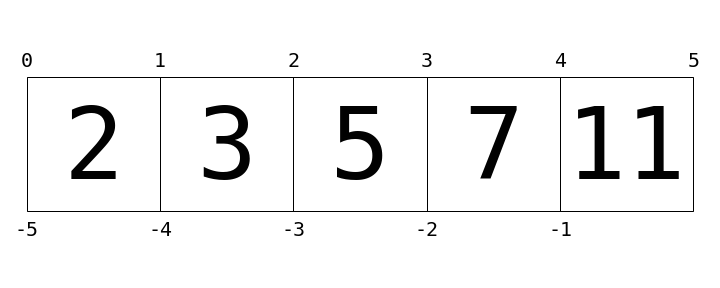
\includegraphics{fig/list-indexing.png}
\caption{List Indexing Figure}
\end{figure}

Here values in the list are represented by large numbers in the squares;
list indices are represented by small numbers above and below. In this
case, \texttt{L{[}2{]}} returns \texttt{5}, because that is the next
value at index \texttt{2}.

Where \emph{indexing} is a means of fetching a single value from the
list, \emph{slicing} is a means of accessing multiple values in
sub-lists. It uses a colon to indicate the start point (inclusive) and
end point (non-inclusive) of the sub-array. For example, to get the
first three elements of the list, we can write:

\begin{Shaded}
\begin{Highlighting}[]
\NormalTok{L[}\DecValTok{0}\NormalTok{:}\DecValTok{3}\NormalTok{]}
\end{Highlighting}
\end{Shaded}

\begin{verbatim}
[2, 3, 5]
\end{verbatim}

Notice where \texttt{0} and \texttt{3} lie in the preceding diagram, and
how the slice takes just the values between the indices. If we leave out
the first index, \texttt{0} is assumed, so we can equivalently write:

\begin{Shaded}
\begin{Highlighting}[]
\NormalTok{L[:}\DecValTok{3}\NormalTok{]}
\end{Highlighting}
\end{Shaded}

\begin{verbatim}
[2, 3, 5]
\end{verbatim}

Similarly, if we leave out the last index, it defaults to the length of
the list. Thus, the last three elements can be accessed as follows:

\begin{Shaded}
\begin{Highlighting}[]
\NormalTok{L[}\OperatorTok{-}\DecValTok{3}\NormalTok{:]}
\end{Highlighting}
\end{Shaded}

\begin{verbatim}
[5, 7, 11]
\end{verbatim}

Finally, it is possible to specify a third integer that represents the
step size; for example, to select every second element of the list, we
can write:

\begin{Shaded}
\begin{Highlighting}[]
\NormalTok{L[::}\DecValTok{2}\NormalTok{]  }\CommentTok{# equivalent to L[0:len(L):2]}
\end{Highlighting}
\end{Shaded}

\begin{verbatim}
[2, 5, 11]
\end{verbatim}

A particularly useful version of this is to specify a negative step,
which will reverse the array:

\begin{Shaded}
\begin{Highlighting}[]
\NormalTok{L[::}\OperatorTok{-}\DecValTok{1}\NormalTok{]}
\end{Highlighting}
\end{Shaded}

\begin{verbatim}
[11, 7, 5, 3, 2]
\end{verbatim}

Both indexing and slicing can be used to set elements as well as access
them. The syntax is as you would expect:

\begin{Shaded}
\begin{Highlighting}[]
\NormalTok{L[}\DecValTok{0}\NormalTok{] }\OperatorTok{=} \DecValTok{100}
\BuiltInTok{print}\NormalTok{(L)}
\end{Highlighting}
\end{Shaded}

\begin{verbatim}
[100, 3, 5, 7, 11]
\end{verbatim}

\begin{Shaded}
\begin{Highlighting}[]
\NormalTok{L[}\DecValTok{1}\NormalTok{:}\DecValTok{3}\NormalTok{] }\OperatorTok{=} \NormalTok{[}\DecValTok{55}\NormalTok{, }\DecValTok{56}\NormalTok{]}
\BuiltInTok{print}\NormalTok{(L)}
\end{Highlighting}
\end{Shaded}

\begin{verbatim}
[100, 55, 56, 7, 11]
\end{verbatim}

A very similar slicing syntax is also used in many data science-oriented
packages, including NumPy and Pandas (mentioned in the introduction).

Now that we have seen Python lists and how to access elements in ordered
compound types, let's take a look at the other three standard compound
data types mentioned earlier.

\subsection{Tuples}\label{tuples}

Tuples are in many ways similar to lists, but they are defined with
parentheses rather than square brackets:

\begin{Shaded}
\begin{Highlighting}[]
\NormalTok{t }\OperatorTok{=} \NormalTok{(}\DecValTok{1}\NormalTok{, }\DecValTok{2}\NormalTok{, }\DecValTok{3}\NormalTok{)}
\end{Highlighting}
\end{Shaded}

They can also be defined without any brackets at all:

\begin{Shaded}
\begin{Highlighting}[]
\NormalTok{t }\OperatorTok{=} \DecValTok{1}\NormalTok{, }\DecValTok{2}\NormalTok{, }\DecValTok{3}
\BuiltInTok{print}\NormalTok{(t)}
\end{Highlighting}
\end{Shaded}

\begin{verbatim}
(1, 2, 3)
\end{verbatim}

Like the lists discussed before, tuples have a length, and individual
elements can be extracted using square-bracket indexing:

\begin{Shaded}
\begin{Highlighting}[]
\BuiltInTok{len}\NormalTok{(t)}
\end{Highlighting}
\end{Shaded}

\begin{verbatim}
3
\end{verbatim}

\begin{Shaded}
\begin{Highlighting}[]
\NormalTok{t[}\DecValTok{0}\NormalTok{]}
\end{Highlighting}
\end{Shaded}

\begin{verbatim}
1
\end{verbatim}

The main distinguishing feature of tuples is that they are
\emph{immutable}: this means that once they are created, their size and
contents cannot be changed:

\begin{Shaded}
\begin{Highlighting}[]
\NormalTok{t[}\DecValTok{1}\NormalTok{] }\OperatorTok{=} \DecValTok{4}
\end{Highlighting}
\end{Shaded}

\begin{verbatim}
---------------------------------------------------------------------------

TypeError                                 Traceback (most recent call last)

<ipython-input-23-141c76cb54a2> in <module>()
----> 1 t[1] = 4


TypeError: 'tuple' object does not support item assignment
\end{verbatim}

\begin{Shaded}
\begin{Highlighting}[]
\NormalTok{t.append(}\DecValTok{4}\NormalTok{)}
\end{Highlighting}
\end{Shaded}

\begin{verbatim}
---------------------------------------------------------------------------

AttributeError                            Traceback (most recent call last)

<ipython-input-24-e8bd1632f9dd> in <module>()
----> 1 t.append(4)


AttributeError: 'tuple' object has no attribute 'append'
\end{verbatim}

Tuples are often used in a Python program; a particularly common case is
in functions that have multiple return values. For example, the
\texttt{as\_integer\_ratio()} method of floating-point objects returns a
numerator and a denominator; this dual return value comes in the form of
a tuple:

\begin{Shaded}
\begin{Highlighting}[]
\NormalTok{x }\OperatorTok{=} \FloatTok{0.125}
\NormalTok{x.as_integer_ratio()}
\end{Highlighting}
\end{Shaded}

\begin{verbatim}
(1, 8)
\end{verbatim}

These multiple return values can be individually assigned as follows:

\begin{Shaded}
\begin{Highlighting}[]
\NormalTok{numerator, denominator }\OperatorTok{=} \NormalTok{x.as_integer_ratio()}
\BuiltInTok{print}\NormalTok{(numerator }\OperatorTok{/} \NormalTok{denominator)}
\end{Highlighting}
\end{Shaded}

\begin{verbatim}
0.125
\end{verbatim}

The indexing and slicing logic covered earlier for lists works for
tuples as well, along with a host of other methods. Refer to the online
\href{https://docs.python.org/3/tutorial/datastructures.html}{Python
documentation} for a more complete list of these.

\subsection{Dictionaries}\label{dictionaries}

Dictionaries are extremely flexible mappings of keys to values, and form
the basis of much of Python's internal implementation. They can be
created via a comma-separated list of \texttt{key:value} pairs within
curly braces:

\begin{Shaded}
\begin{Highlighting}[]
\NormalTok{numbers }\OperatorTok{=} \NormalTok{\{}\StringTok{'one'}\NormalTok{:}\DecValTok{1}\NormalTok{, }\StringTok{'two'}\NormalTok{:}\DecValTok{2}\NormalTok{, }\StringTok{'three'}\NormalTok{:}\DecValTok{3}\NormalTok{\}}
\end{Highlighting}
\end{Shaded}

Items are accessed and set via the indexing syntax used for lists and
tuples, except here the index is not a zero-based order but valid key in
the dictionary:

\begin{Shaded}
\begin{Highlighting}[]
\CommentTok{# Access a value via the key}
\NormalTok{numbers[}\StringTok{'two'}\NormalTok{]}
\end{Highlighting}
\end{Shaded}

\begin{verbatim}
2
\end{verbatim}

New items can be added to the dictionary using indexing as well:

\begin{Shaded}
\begin{Highlighting}[]
\CommentTok{# Set a new key:value pair}
\NormalTok{numbers[}\StringTok{'ninety'}\NormalTok{] }\OperatorTok{=} \DecValTok{90}
\BuiltInTok{print}\NormalTok{(numbers)}
\end{Highlighting}
\end{Shaded}

\begin{verbatim}
{'three': 3, 'ninety': 90, 'two': 2, 'one': 1}
\end{verbatim}

Keep in mind that dictionaries do not maintain any sense of order for
the input parameters; this is by design. This lack of ordering allows
dictionaries to be implemented very efficiently, so that random element
access is very fast, regardless of the size of the dictionary (if you're
curious how this works, read about the concept of a \emph{hash table}).
The \href{https://docs.python.org/3/library/stdtypes.html}{python
documentation} has a complete list of the methods available for
dictionaries.

\subsection{Sets}\label{sets}

The fourth basic collection is the set, which contains unordered
collections of unique items. They are defined much like lists and
tuples, except they use the curly brackets of dictionaries:

\begin{Shaded}
\begin{Highlighting}[]
\NormalTok{primes }\OperatorTok{=} \NormalTok{\{}\DecValTok{2}\NormalTok{, }\DecValTok{3}\NormalTok{, }\DecValTok{5}\NormalTok{, }\DecValTok{7}\NormalTok{\}}
\NormalTok{odds }\OperatorTok{=} \NormalTok{\{}\DecValTok{1}\NormalTok{, }\DecValTok{3}\NormalTok{, }\DecValTok{5}\NormalTok{, }\DecValTok{7}\NormalTok{, }\DecValTok{9}\NormalTok{\}}
\end{Highlighting}
\end{Shaded}

If you're familiar with the mathematics of sets, you'll be familiar with
operations like the union, intersection, difference, symmetric
difference, and others. Python's sets have all of these operations
built-in, via methods or operators. For each, we'll show the two
equivalent methods:

\begin{Shaded}
\begin{Highlighting}[]
\CommentTok{# union: items appearing in either}
\NormalTok{primes }\OperatorTok{|} \NormalTok{odds      }\CommentTok{# with an operator}
\NormalTok{primes.union(odds) }\CommentTok{# equivalently with a method}
\end{Highlighting}
\end{Shaded}

\begin{verbatim}
{1, 2, 3, 5, 7, 9}
\end{verbatim}

\begin{Shaded}
\begin{Highlighting}[]
\CommentTok{# intersection: items appearing in both}
\NormalTok{primes }\OperatorTok{&} \NormalTok{odds             }\CommentTok{# with an operator}
\NormalTok{primes.intersection(odds) }\CommentTok{# equivalently with a method}
\end{Highlighting}
\end{Shaded}

\begin{verbatim}
{3, 5, 7}
\end{verbatim}

\begin{Shaded}
\begin{Highlighting}[]
\CommentTok{# difference: items in primes but not in odds}
\NormalTok{primes }\OperatorTok{-} \NormalTok{odds           }\CommentTok{# with an operator}
\NormalTok{primes.difference(odds) }\CommentTok{# equivalently with a method}
\end{Highlighting}
\end{Shaded}

\begin{verbatim}
{2}
\end{verbatim}

\begin{Shaded}
\begin{Highlighting}[]
\CommentTok{# symmetric difference: items appearing in only one set}
\NormalTok{primes }\OperatorTok{^} \NormalTok{odds                     }\CommentTok{# with an operator}
\NormalTok{primes.symmetric_difference(odds) }\CommentTok{# equivalently with a method}
\end{Highlighting}
\end{Shaded}

\begin{verbatim}
{1, 2, 9}
\end{verbatim}

Many more set methods and operations are available. You've probably
already guessed what I'll say next: refer to Python's
\href{https://docs.python.org/3/library/stdtypes.html}{online
documentation} for a complete reference.

\subsection{More Specialized Data
Structures}\label{more-specialized-data-structures}

Python contains several other data structures that you might find
useful; these can generally be found in the built-in
\texttt{collections} module. The collections module is fully-documented
in \href{https://docs.python.org/3/library/collections.html}{Python's
online documentation}, and you can read more about the various objects
available there.

In particular, I've found the following very useful on occasion:

\begin{itemize}
\tightlist
\item
  \texttt{collections.namedtuple}: Like a tuple, but each value has a
  name
\item
  \texttt{collections.defaultdict}: Like a dictionary, but unspecified
  keys have a user-specified default value
\item
  \texttt{collections.OrderedDict}: Like a dictionary, but the order of
  keys is maintained
\end{itemize}

Once you've seen the standard built-in collection types, the use of
these extended functionalities is very intuitive, and I'd suggest
\href{https://docs.python.org/3/library/collections.html}{reading about
their use}.

\end{document}
